\documentclass[convert={density=1200}]{standalone}
\usepackage{tikz}
\usetikzlibrary{shapes.geometric, arrows, matrix, positioning, automata, backgrounds}

\tikzstyle{server} = [rectangle, rounded corners, text centered, draw=black, fill=green!30, inner sep=5pt]
\tikzstyle{node} = [rectangle, rounded corners, text centered, draw=black, fill=blue!30, inner sep=5pt]
\tikzstyle{action} = [rectangle, text centered, draw=black, fill=white, inner sep=5pt]
\tikzstyle{virtual} = [trapezium, text centered, draw=black, fill=yellow!30, inner sep=5pt, text=red!50!black, font=\ttfamily]

\tikzstyle{server_message} = [thick, green!50!black, dashed,->, >=stealth]
\tikzstyle{node_message} = [thick, blue, dashed, ->, >=stealth]
\tikzstyle{action_step} = [thick, black, ->, >=stealth]

\begin{document}

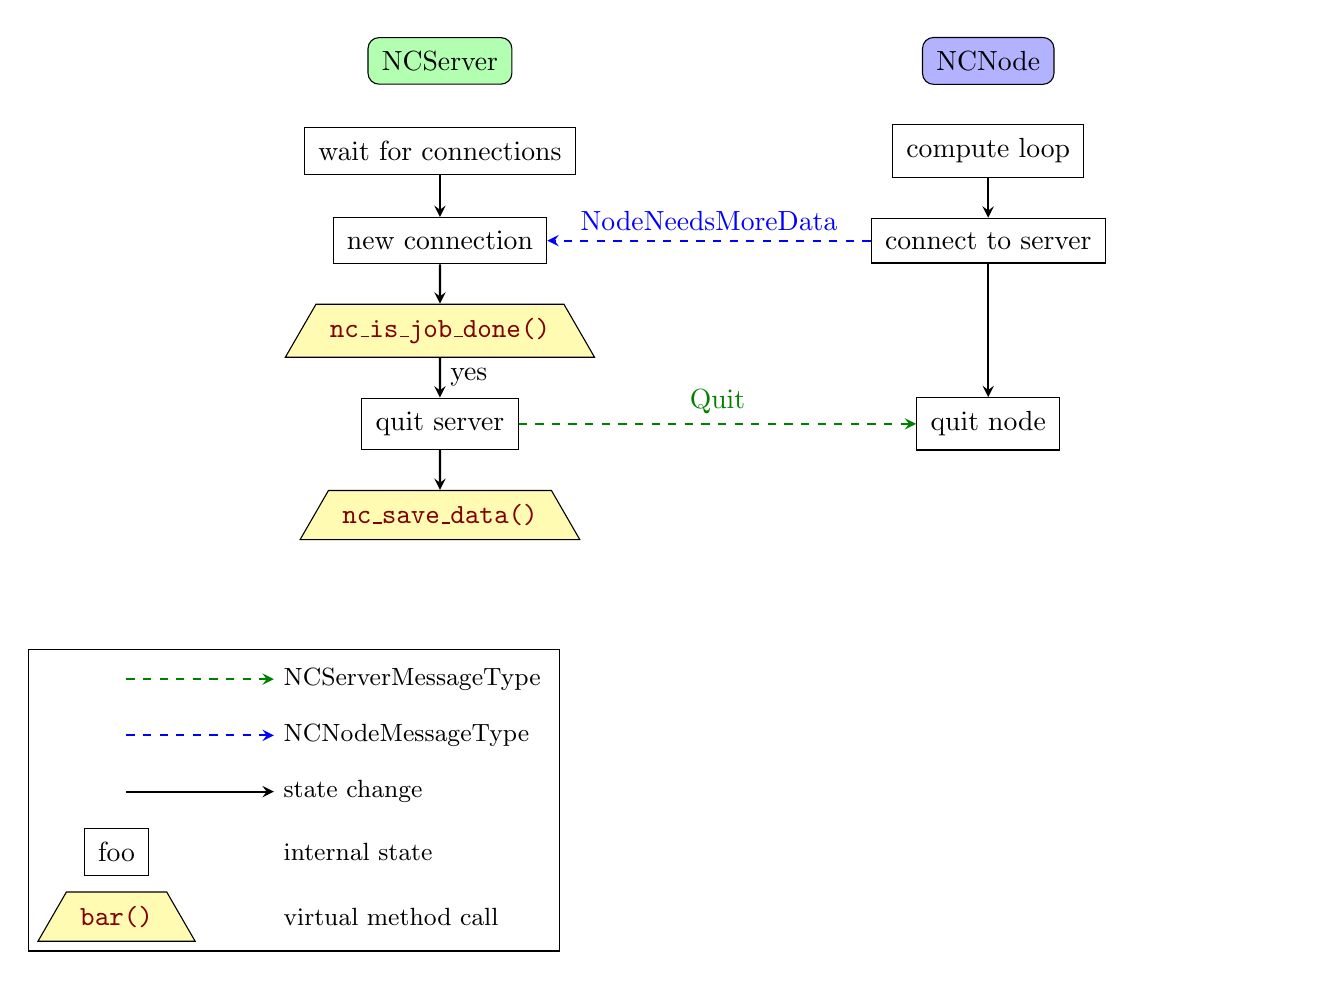
\begin{tikzpicture}

    \matrix [column sep = 35mm, row sep = 5mm] {
        \node (ncserver) [server] {NCServer}; &
        \node (ncnode) [node] {NCNode}; \\

        \node (wait) [action] {wait for connections}; &
        \node (loop) [action] {compute loop}; \\

        \node (connected1) [action] {new connection}; &
        \node (connect1) [action] {connect to server}; \\

        \node (job_done) [virtual] {nc\_is\_job\_done()}; & \\

        \node (quit_server) [action] {quit server}; &
        \node (quit_node) [action] {quit node}; \\

        \node (save_data) [virtual] {nc\_save\_data()}; & \\
    };

    \draw [action_step] (wait) -- (connected1);
    \draw [action_step] (connected1) -- (job_done);
    \draw [action_step] (job_done) -- node [right, text width=2.5cm] {yes} (quit_server);
    \draw [action_step] (quit_server) -- (save_data);

    \draw [action_step] (loop) -- (connect1);
    \draw [node_message] (connect1) -- node [above] {NodeNeedsMoreData} (connected1);
    \draw [server_message] (quit_server) -- node [above] {Quit} (quit_node);
    \draw [action_step] (connect1) -- (quit_node);

    % Add bottom page border with invisible node
    \node at (0, -8.5) {};

    % Add left page border with invisible node
    \node at (-8.2, 0) {};

    % Add right page border with invisible node
    \node at (7.7, 0) {};

    \matrix [column sep=10mm, row sep=2.0mm, rectangle, draw=black,
             column 2/.style={anchor=west}
        ] at (-5.1, -6.5) {
        \node (label1a) {}; & \node [font=\small] (label1b) {NCServerMessageType}; \\
        \node (label2a) {}; & \node [font=\small] (label2b) {NCNodeMessageType}; \\
        \node (label3a) {}; & \node [font=\small] (label3b) {state change}; \\
        \node [action] {foo}; & \node [font=\small] {internal state}; \\
        \node [virtual] {bar()}; & \node [font=\small] {virtual method call}; \\
    };

    \draw [server_message] (label1a) -- (label1b);
    \draw [node_message] (label2a) -- (label2b);
    \draw [action_step] (label3a) -- (label3b);

\end{tikzpicture}

\end{document}
